\documentclass[discrete.tex]{subfiles}

\begin{document}
  \section{Алгоритм поиска контура и построение диаграммы порядка}

  \begin{task}
    Построить граф $<M_s,N_s>$, где элементами $M_s$ являются компоненты сильной связности графа $<M,N,T>$, а дугами - те дуги графа $<M,N,T>$, концы которых принадлежат разным компонентам. Кроме того, отождествим дуги с одинаковым началом и концом. Такой граф назовем диаграммой порядка (графом Герца) графа $<M,N,T>$
  \end{task}

  \begin{ttheorem}
    Граф компонент сильной связности (диаграмма порядка) не имеет контуров
  \end{ttheorem}

  \begin{pproof}
    *здесь когда-нибудь будет док-во*
  \end{pproof}

  \begin{alg}[поиска контура]
    Состояние вычислительного процесса. Граф $<M_0, N_0>$ и простой путь $<M',N'>$

    Начальное состояние. $M_0 = M,\q N_0 = N$, путь состоит из любой вершины $i_0 \in M$

    Стандартный шаг: Пусть k - длина пути, $i_k$ - конец пути. Рассмотрим множество дуг из $N_0$, для которых вершина $i_k$ является началом:
    \[N^-(i_k) = \{j \in N_0 | \beg j = i_k\}\]
    Если мн-во $N^-(i_k)$ не пусто, выберем в нем произвольную дугу, обозначим её через $j_{k+1}$, а её конец через $i_{k+1}$. Если нет, то увеличим k на единицу, нарастив путь $<M', N'>$

    Если мн-во $N^-(i_k)$ пусто, объявим вершину $i_k$ тупиковой и удалим её из $M_0$, а из $N_0$ удалим все дуги, для которых $i_k$ является концом. Путь $<M',N'>$, при этом следует уменьшить на одну дугу, если $k>0$, а если $k=0$, нужно искать очередную вершину, ещё оставшуюся в мн-ве $M_0$
  \end{alg}

  \begin{alg}[построения диаграммы порядка]
    Модифицируем предыдущий алгоритм. Заменим вершины графа на укрупненные, состав которых изменяется в ходе вычислений. Для каждой укрепленной вершины перебираются дуги, выходящие из вершин, составляющих эту укрепленную вершину. Дуги, привратившиеся из-за укрепления в петли игнорируются
  \end{alg}

  \begin{example}\
    \begin{figure}[H]
            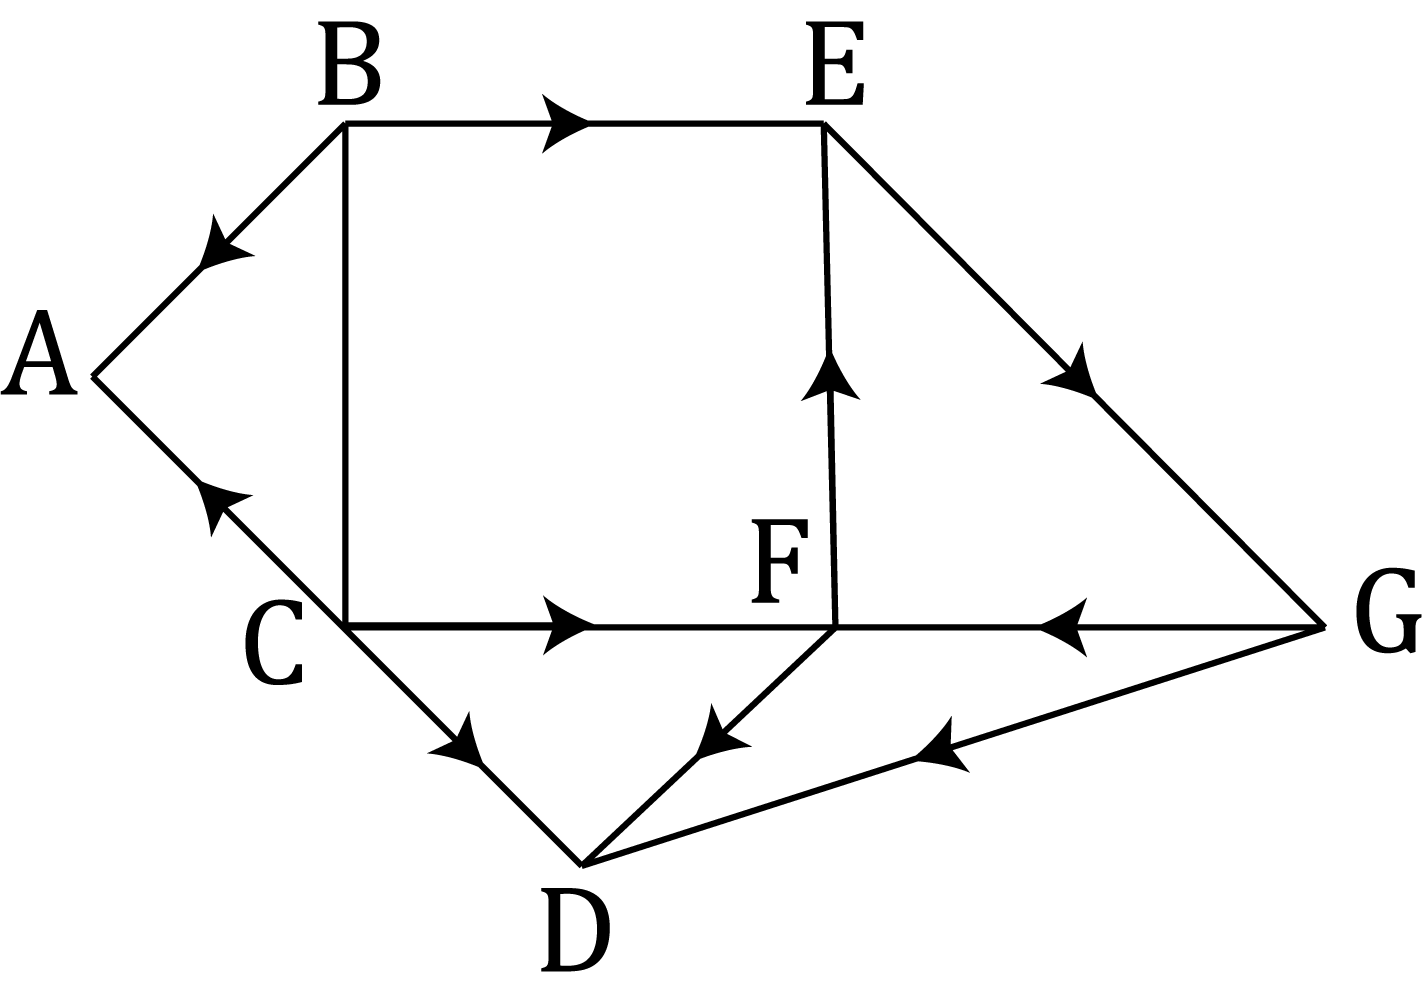
\includegraphics[width=5cm]{pics/39_1}
            \centering
    \end{figure}
    \begin{enumerate}
      \item R(A)
      \item R(A, B)
      \item R(A, B, C)
      \item R(A, B, C, A) - контур
      \item R((ABC), D) - тупик
      \item R((ABC), F)
      \item R((ABC), F, D) - тупик
      \item R((ABC), F, E)
      \item R((ABC), F, E, G)
      \item R((ABC), F, E, G, D) - тупик
      \item R((ABC), F, E, G, F) - контур
      \item R((ABC), (F, E, G)) - уде были (через BE)
    \end{enumerate}
    \begin{figure}[H]
            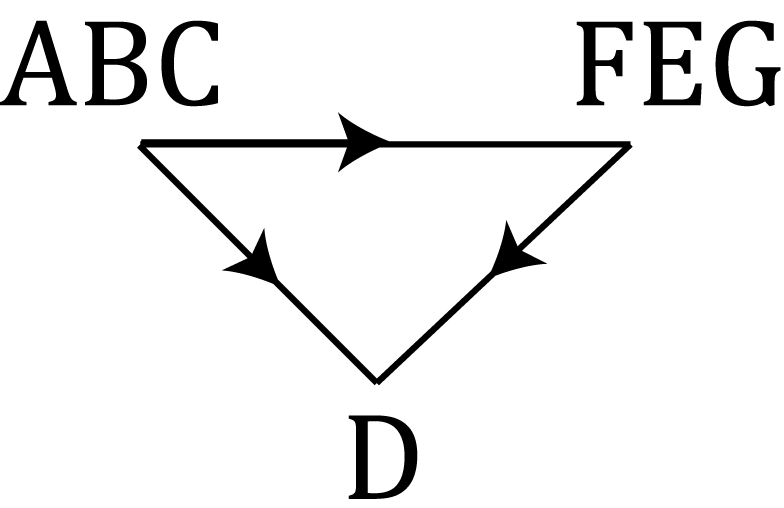
\includegraphics[width=3cm]{pics/39_2}
            \centering
    \end{figure}
  \end{example}
\end{document}
